\input{../common}
\everymath{\displaystyle}
\begin{document}
  %<*content>
  \lesson{algebra}{8}{Probabilités  conditionnelles}
  
  \begin{lemma}
  Dans une classe de 40 élèves, les 25 sont des garçons.\\ 10 garçons et 5 filles ont la moyenne à l'issue d'une composition. \\On choisit au hasard un élève de cette classe. On considère les événements suivants:\\ G: << l'élève choisi est un garçon.>>  $ \quad $
 M: << l'élève choisi a la moyenne.>>
\begin{enumerate}
\item Décrire l'événement G$ \cap $M.
\item Donner les valeurs de P(G), P(M) et P( G$ \cap $M).
\item On choisit  un élève parmi les garçons. Quelle est la probabilité qu'il ait la moyenne ? \\On note cette probabilité par P(M/G).
\item Comparer P(M/G) \;et \;$ \dfrac{P( G \cap M)}{P(G)} $
\end{enumerate}
  \end{lemma}
  \subsection{Définition et propriétés}
\begin{definition}
Soient $A$ et $B$ deux événements de l'univers $ \Omega $ d'une expérience aléatoire avec $ P(A)\neq 0 $.\\On appelle \textbf{probabilité conditionnelle de $B$ sachant que $A$ est réalisé}, le nombre: \\

$ P(B/A)=\dfrac{P( A \cap B)}{P(A)}   \hspace*{1cm}$ (\textit{l'univers se réduit à $A$} )


\medskip


Le nombre réel  $P(B/A)$ se note aussi $P_{A}(B)$.
\end{definition}

\begin{example}
On lance un dé équilibré à six faces numérotées de 1 à 6.\\
 $ \bullet $ Si A est l'événement  << \textbf{le résultat est pair}>>,  on a\;  $ P _{A}(\accol{2})=\dfrac{\dfrac{1}{6}}{\dfrac{1}{2}} =\dfrac{1}{3}$\; et \;$P _{A}(\accol{5})=0  $ \\

 $ \bullet $ Si B désigne  l'événement  << \textbf{le résultat est un multiple de 3}>>,  on a\\

 B$ =\accol{3; 6} $\; et \;  $ P _{A}(B)=\dfrac{P(\accol{6})}{P(A)} =\dfrac{1}{3}$
\end{example}
\begin{theorem}
L'application  qui, à tout événement B associe le réel P$ _{A} $(B) définit une probabilité sur $ \Omega $ , appelée \textbf{probabilité conditionnelle sachant  A}.

\end{theorem}



\textbf{Démonstration}\\
P$ _{A} $ associe à tout événement un réel positif, et on a P$ _{A}(\varnothing)=0 $\\
De plus, si $ \accol{x} $   est un événement élémentaire dans $ \Omega $, par définition de P$ _{A} $, on a: si $x \notin $A, alors P$ _{A}(\accol{x})=0 $.\\

Ainsi $ \displaystyle\sum_{x\in \Omega} P _{A}(\accol{x}) = \displaystyle\sum_{x\in A} P _{A}(\accol{x})=\displaystyle\sum_{x\in A} \dfrac{P(\accol{x})}{P(A)}=\dfrac{1}{P(A)}\displaystyle\sum_{x\in A}P(\accol{x})=\dfrac{1}{P(A)}\times P(A)=1$\\
 On peut donc conclure que  $P_{A}(B)$ est une probabilité sur $ \Omega $.
 
 \begin{property}
 Si $A$ est un événement de probabilité non nul et $B$ un événement quelconque dans l'univers $ \Omega $, on a:

\begin{enumerate}
\item $ PA\cap B=P(A)\times P_{A}(B)$
\item Si $A$ et $B$ sont \textbf{incompatibles}, P$_{A}(B) =0 $
\item $P_{A}(A) =1 $
\item  $P_{A}(\overline{B}) =1- P_{A}(B)$
\end{enumerate}
 \end{property}
 
Les démonstrations sont immédiates à partir de la définition de  P$ _{A} $.
\subsection{Probabilités conditionnelles et arbre de pondéré}


 Pour   modéliser  une situation de probabilités conditionnelles,  on utilise  souvent un arbre  pondéré  dans lequel s'applique  le principe multiplicatif  qui découle de l'égalité:\; $P A\cap B=P(A) \times P_{A}(B)$.\\ Si par exemple dans une expérience aléatoire  on considère la réalisation ou non d'un événement A   puis  la réalisation d'un autre événement B alors on peut représenter la situation par l'arbre ci-dessous.\\ Les probabilités figurant sur les sous branches sont des probabilités conditionnelles. 
 
 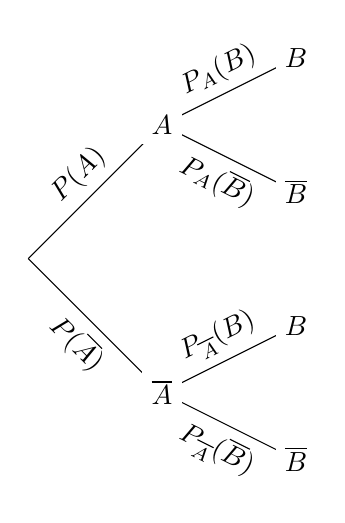
\begin{tikzpicture}[xscale=0.85,yscale=0.85]
\draw (-2,0.5)--(-4,1.5) node[midway, below, sloped]{$ P _{\overline{A}} (\overline{B})$};
 \draw (-2,2.5)--(-4,1.5) node[midway, above, sloped]{$ P _{\overline{A}} (B)  $};
 \draw (-2,4.5)--(-4,5.5) node[midway, below, sloped]{$P _{A} (\overline{B})   $};
 \draw (-2,6.5)--(-4,5.5) node[midway, above, sloped]{$ P _{A} (B) $};
 \draw (-4,1.5)--(-6,3.5) node[midway, below, sloped]{$ P(\overline{A}) $};
 \draw (-4,5.5)--(-6,3.5) node[midway, above, sloped]{$ P(A) $};
 \draw (-2,0.5) node[fill=white]{$\overline{B}$};
 \draw (-2,2.5) node[fill=white]{$B$};
 \draw (-2,4.5) node[fill=white]{$\overline{B}$};
 \draw (-2,6.5) node[fill=white]{$B$};
 \draw (-4,1.5) node[fill=white]{$\overline{A}$};
 \draw (-4,5.5) node[fill=white]{$A$};
 \end{tikzpicture}

  \subsection{Formule des probabilités totales}
\begin{theorem}
Soient  A$ _{1} $,  A$ _{2} \;  \cdots   $ \; A$ _{n} $  des événements formant une partition de $ \Omega $  et B un événement quelconque de $ \Omega $.  On a: 
$$ P(B)= P(A_{1}) \times P_{A_{1}}(B)+P(A_{2}) \times P_{A_{2}}(B)+\;\cdots\;  +P(A_{n}) \times P_{A_{n}}(B)$$

\end{theorem}

\textbf{Démonstration}\\
B est la réunion des événements B$ \cap A_{1} $,  B$ \cap A_{1} $, \;$ \cdots $\; B$ \cap A_{n} $,  qui sont  deux à deux disjoints.  Ainsi:\\
P(B)$ = P(B\cap A_{1})+P(B\cap A_{2}) +\;\cdots\;  +P(B\cap A_{n})$\\
 Or pour tout $ i\in\accol{1; 2; \cdots ;\; n} $;\;\;  $P(B\cap A_{i})= P(A_{i}) \times P_{A_{i}}(B) $\\
  D'où:  \;\; $P(B) = P(A_{1}) \times P_{A_{1}}(B)+P(A_{2}) \times P_{A_{2}}(B)+\;\cdots\;  +P(A_{n}) \times P_{A_{n}}(B)$\\
  
  \textbf{Un cas particulier très utilisé} $ \; P(B) = P(A) \times P(B/A)+P(\overline{A}) \times P\paren{B/\overline{A}} \; $ (Voir arbre pondéré)
  
  \subsection{Indépendance deux événements}
 \begin{definition}
Soit P une probabilité sur un univers $ \Omega $.\\
On dit que \textbf {les événements A et B sont indépendants} si,\quad 
$ P(A\cap B)= P(A)\times  P(B)$
 \end{definition}
\begin{example}
Dans le lancer d'un dé équilibré à six faces, les événements A: << le résultat est pair >>  et  B : << le résultat est 2 >>   ne sont pas indépendants.\\ En effet $ P(A\cap B)=\frac{1}{6} $\; et \; $P(A)\times  P(B)= \frac{1}{2}\times\frac{1}{6} \quad$.  Donc  $P(A)\times  P(B)\neq \frac{1}{6} $\\
Si C est l'événement : << le résultat est supérieur ou égal à 5 >> , alors les événements A et C sont indépendants.\\
\end{example}
\begin{property}
On suppose  P$ (A)\neq 0 $.\\
 A et B sont indépendants si, et seulement si, $\;P _{A}(B)=P(B) $
\end{property}
\textbf{Démonstration}\\
On suppose   P$ (A)\neq 0 \;$.  On alors  $ P(A\cap B)= P(A)\times  P_{A}(B)$\\
 A et B sont indépendants si, et seulement si:\quad 
 $ P(A)\times  P_{A}(B)= P(A)\times  P(B)$\\ C'est-à-dire $ P_{A}(B)= P(B)$,\; en simplifiant par \;  P$ (A)\neq 0 $.
\begin{exercice}
  Afin d'équiper les élèves des groupes scolaires de la commune, une municipalité achète auprès d'un grossiste des stylos-billes de trois marques différentes, A, B et C.\\
  $ \bullet \; $  40\%  des stylos commandés sont de marques A,  la moins chère ; parmi ces stylos, 15\% sont défectueux.\\
$ \bullet \; $ 35\%  des stylos commandés sont de marques B et \; 10\% sont défectueux.\\
 $ \bullet \; $ 25\%  des stylos commandés sont de marques C et \; 5\% sont défectueux.\\ On choisit  hasard  un stylo dans le stock de la  municipalité.
  \begin{enumerate}
  \item Construire un arbre pondéré décrivant la situation étudiée.
  \item Déterminer la probabilité que le stylo choisi soit défectueux.
  \item Le stylo choisi est en bon état de fonctionnement.
  Quelle est la probabilité, au centième près, qu'il soit de marque C ?
 \end{enumerate}
\end{exercice}
\begin{proof}
 \begin{enumerate}
  \item 
     On construit un arbre pondéré dont les branches de premier niveau aboutissent aux  événements A, B et C. En effet l'énoncé donne les probabilités   de ces événements  puis  ensuite les probabilités conditionnelles  sachant que l'un de ces événements est réalisé.\;On adopte  les notations A ( respectivement B, C):\; << le stylo  choisi est de marque A>>,(respectivement B, C); \; D\;<< le stylo choisi est défectueux>>.
  
    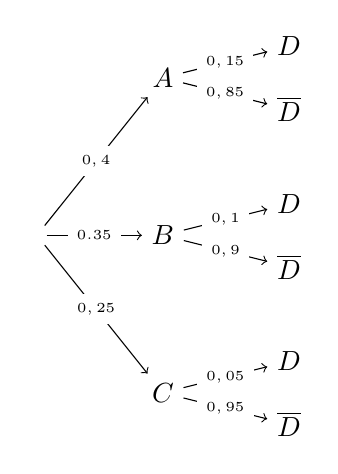
\begin{tikzpicture}[grow=right,level distance=2cm,scale=0.8,
                        level 1/.style={sibling distance=2.5cm},
                        level 2/.style={sibling distance=1cm}]
    \tikzstyle{edge from parent}=[->,draw]
    \tikzstyle{arrete}=[fill=white,font=\tiny]
    \tikzstyle{noeud}=[draw,ellipse]
    \node {}
       child {node {$C$}
          child {node {$\overline{D}$}
          edge from parent node[arrete] {$0,95$}}
         % child {node {$V$}
         % edge from parent node[arrete] {$3/9$}}
          child {node {$D$}
          edge from parent node[arrete] {$0,05$}}
       edge from parent node[arrete] {$0,25$}
       }
       child {node {$B$}
          child {node {$\overline{D}$}
          edge from parent node[arrete] {$0,9$}}
         % child {node {$V$}
          %edge from parent node[arrete] {$3/9$}}
          child {node {$D$}
          edge from parent node[arrete] {$0,1$}}
       edge from parent node[arrete] {$0.35$}
       }
       child {node {$A$}
          child {node {$\overline{D}$}
          edge from parent node[arrete] {$0,85$}}
         % child {node {$V$}
         % edge from parent node[arrete] {$3/9$}}
          child {node {$D$}
          edge from parent node[arrete] {$0,15$}}
       edge from parent node[arrete] {$0,4$}
       };
    \end{tikzpicture}
   

\item   Les événements  A, B, C  forment une partition de l'univers des choix possibles\;( en effet ils sont de probabilités non nulles, et incompatibles deux à deux car un stylo ne peut-être de deux marques  différentes  et leur réunion couvre tous les cas possibles). On peut  donc appliquer la formule des probabilités totales  pour calculer la probabilité P(D). \\

P(D)$ =P(A)\times P_{A}(D)+P(B)\times P_{B}(D)+P(C)\times P_{C}(D)$\\

On obtient \;P(D)$ = 0,4\times 0,15  + 0,35\times 0,1+0,25\times0,05 =0,1075$
\item On cherche ici à calculer  la probabilité  P$ _{\overline{D}}(C) $.\\
On applique la définition d'une probabilité conditionnelle.\\

P$ _{\overline{D}}(C)=\dfrac{P(\overline{D}\cap C)}{P(\overline{D})} $\\
Le calcul de \; $ P(\overline{D}\cap C )$ \; s'obtient en appliquant le principe multiplicatif  dans la branche la plus basse de l"arbre pondéré construit à la question 1) $\; P(\overline{D}\cap C )= P(C)\times P_{C}(\overline{D})= 0,95 \times 0,25$ \\

Ainsi , \; $ P(\overline{D}\cap C )=0,2375 $ \; et\;  P$ _{\overline{D}}(C)=\dfrac{0,2375}{1-0,1075}$ ,\;  soit \; $ 0,27 $\; au centième près.
\end{enumerate}


\end{proof}
  %</content>
\end{document}
